\section*{Question 7:}
Exercise 9.9: Use K-means and spherical K-means to cluster the data points in Exercise 9.8. How do the clusterings differ?

\subsection*{Answer:}

The data points from Exercise 9.8 are:
$$(-4,-2),(-3,-2),(-2,-2),(-1,-2),(1,-1),(1,1),(2,3),(3,2),(3,4),(4,3)$$


I wrote two simple python scripts to cluster the data points, ``k.py'' and ``sk.py'', using K-means and spherical K-means respectively.
I ran both programs for k = 2, 3, and 4.

The programs also generate plots for the data before and after clustering.

\subsection{K-means:}

\lstinputlisting[language=Python, breakatwhitespace=〈false), label=The content of k.py, caption= The content of k.py]{Q7/k.py}

\begin{lstlisting}[breakatwhitespace=〈false)]
hussam@hussam-HP-Compaq-nc8430-GE542UP-ABA:~/Desktop/99$ python k.py 2
hussam@hussam-HP-Compaq-nc8430-GE542UP-ABA:~/Desktop/99$ python k.py 3
hussam@hussam-HP-Compaq-nc8430-GE542UP-ABA:~/Desktop/99$ python k.py 4
\end{lstlisting}

\begin{figure}[h]
\caption{K-means for K = 1}
\centering
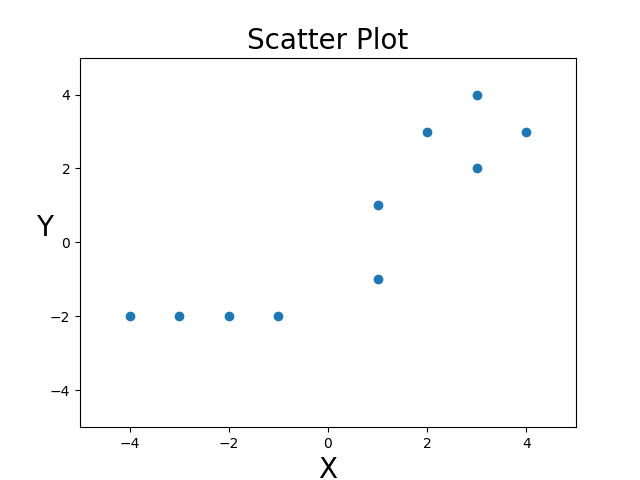
\includegraphics[scale=0.8]{Q7/k1.png}
\end{figure}

\pagebreak

\begin{figure}[h]
\caption{K-means for K = 2}
\centering
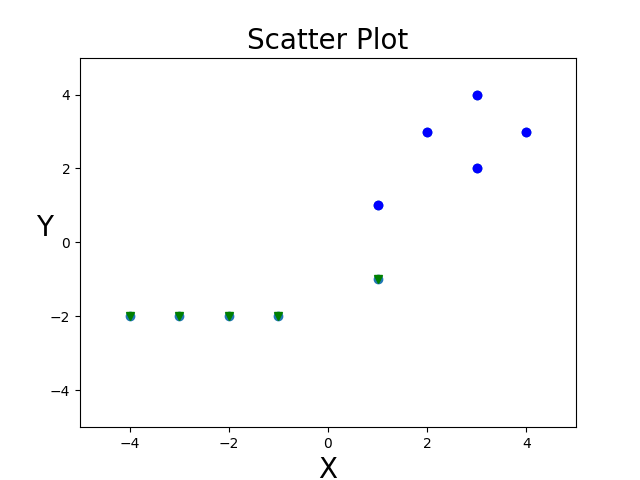
\includegraphics[scale=0.8]{Q7/k2.png}
\end{figure}

\pagebreak

\begin{figure}[h]
\caption{K-means for K = 3}
\centering
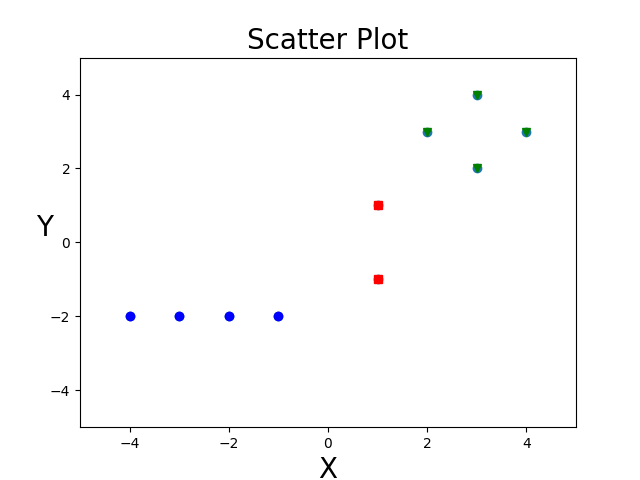
\includegraphics[scale=0.8]{Q7/k3.png}
\end{figure}

\pagebreak

\begin{figure}[h]
\caption{K-means for K = 4}
\centering
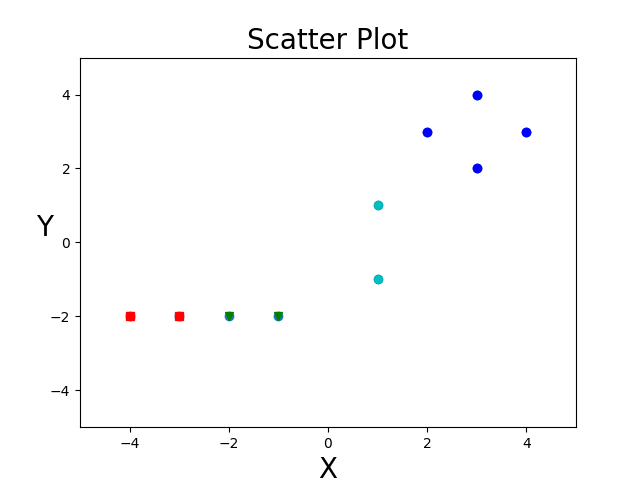
\includegraphics[scale=0.8]{Q7/k4.png}
\end{figure}

\pagebreak

\subsection{Spherical K-means:}

\lstinputlisting[language=Python, breakatwhitespace=〈false), label=The content of sk.py, caption= The content of sk.py]{Q8/sk.py}

\begin{lstlisting}[breakatwhitespace=〈false)]
hussam@hussam-HP-Compaq-nc8430-GE542UP-ABA:~/Desktop/99$ python sk.py 4
hussam@hussam-HP-Compaq-nc8430-GE542UP-ABA:~/Desktop/99$ python sk.py 3
hussam@hussam-HP-Compaq-nc8430-GE542UP-ABA:~/Desktop/99$ python sk.py 2
\end{lstlisting}

\pagebreak

\begin{figure}[h]
\caption{Spherical K-means for K = 2}
\centering
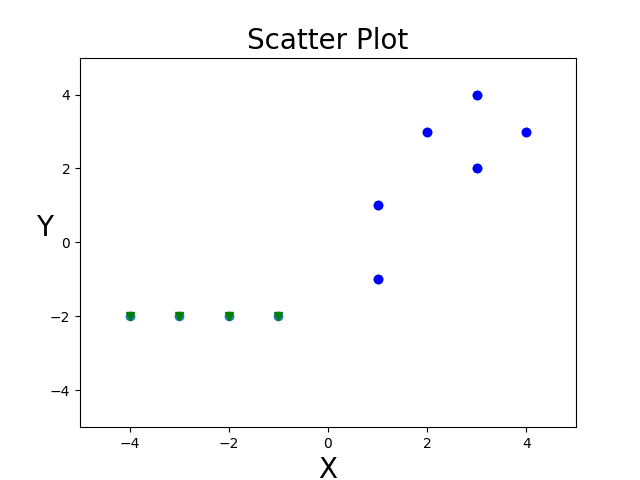
\includegraphics[scale=0.8]{Q7/sk2.png}
\end{figure}

\pagebreak

\begin{figure}[h]
\caption{Spherical K-means for K = 3}
\centering
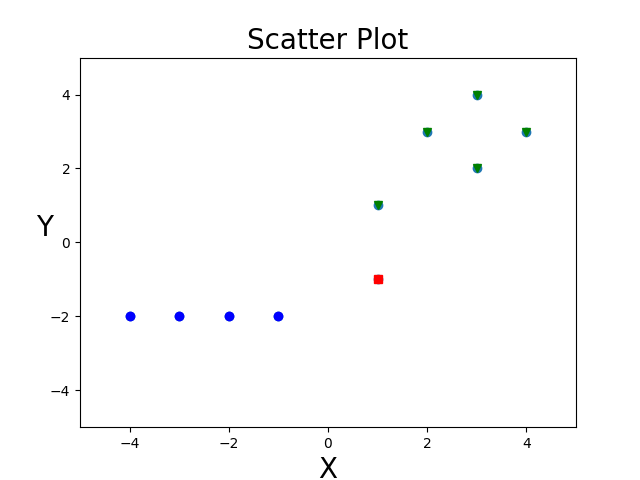
\includegraphics[scale=0.8]{Q7/sk3.png}
\end{figure}

\pagebreak

\begin{figure}[h]
\caption{Spherical K-means for K = 4}
\centering
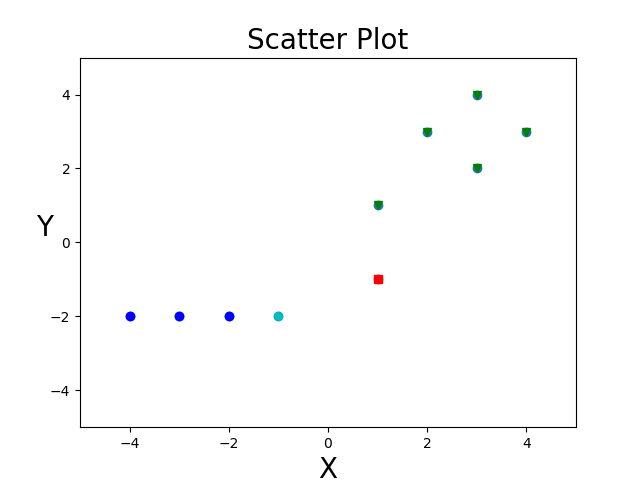
\includegraphics[scale=0.8]{Q7/sk4.png}
\end{figure}

\pagebreak


\textbf{Observation:}

K-means and Spherical K-means produced different results for all tested K values. The reason is that each clustering algorithm has a different approach to solve the clustering problem. K-means minimizes the Euclidean distance between the cluster center and the members of the cluster. The intuition behind this is that the radial distance from the cluster center to the element location should be similar for all elements of that cluster. On the other hand, Sperical K-means sets the center of the cluster such that it makes both uniform and minimal angle between components. The points should have consistent spacing between each other. That spacing is simpler to quantify as cosine similarity. 